\documentclass{article}
\usepackage{geometry}
\usepackage{graphicx}
\usepackage{amsmath}
\usepackage{algorithm}
\usepackage{algpseudocode}
\usepackage{dsfont}
\usepackage{amssymb}
\usepackage{multicol}

\geometry{
a4paper,
right=10mm,
left=10mm,
top=10mm,
bottom=10mm,	
}

\begin{document}

\pagenumbering{gobble}

\begin{center}
\textbf{\Large Assignment 1 : CS785} \\
\textit{\large Jayant Agrawal}         14282
\end{center}

\section{Car Accident}
\textbf{(a)} \\
Consider the following game tree for the car accident(Figure \ref{1_gt1}). Here \emph{5000C} represents that Ram gave Rahim 5000, \emph{5000R} represents that Ram asked Rahim for a receipt of 5000 and \emph{2500C,2500R} represents that Ram gave half the amount and expected the receipt for the other half. For Rahim, R represents 'repair' and NR represents 'not repair'. Also, we are assuming that Ram has already lost his 5000, and whatever he saves is his payoff.
\begin{figure}[h!]
\begin{center}
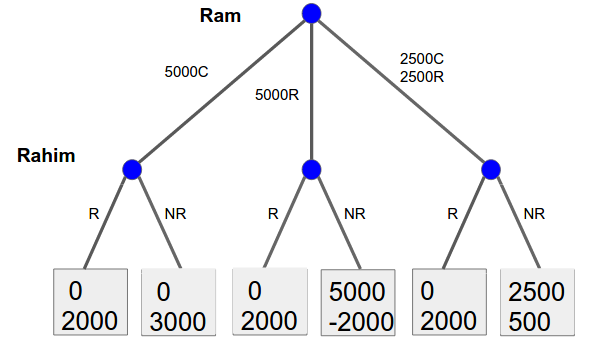
\includegraphics[scale=0.4]{1_gt1.png}
\label{1_gt1}
\caption{Game Tree: Car Accident}
\end{center}
\end{figure} \\
\textbf{(b)} 5000C $\rightarrow$ C , 5000R $\rightarrow$ R, 2500C,2500R $\rightarrow$ CR, R $\rightarrow$ r, NR $\rightarrow$ n\\ \\
\begin{center}
\begin{tabular}{|c|c|c|c|c|c|c|c|c|}
\hline
& $C_rR_rCR_r$ & $C_rR_rCR_n$ & $C_rR_nCR_r$ & $C_nR_rCR_r$ & $C_rR_nCR_n$ & $C_nR_nCR_r$ & $C_nR_rCR_n$ & $C_nR_nCR_n$ \\
\hline
\textbf{C} & 0,2000 & 0,2000 & 0,2000 & 0,3000 & 0,2000 & 0,3000 & 0,3000 & 0,3000 \\
\hline
\textbf{R} & 0,2000 & 0,2000 & 5000,-2000 & 0,2000 & 5000,-2000 & 5000,-2000 & 0,2000 & 5000,-2000 \\
\hline
\textbf{CR} & 0,2000 & 2500,500 & 0,2000 & 0,2000 & 2500,500 & 0,2000 & 2500,500 & 2500,500 \\
\hline
\end{tabular} 
\end{center}
\textbf{(c)} \\
For the above clearly, Nash Equilibrium is at following: \\
\{C,$C_nR_rCR_r$\} \\
\{R,$C_rR_rCR_r$\} \\
\{R,$C_nR_rCR_r$\} \\
\{CR,$C_rR_rCR_r$\} \\
\{CR,$C_nR_rCR_r$\} \\

\textbf{(d)} Using Backward Induction: \\
Rahim argues, that if Ram chooses \emph{5000C}, then the best response is \emph{NR}. If Ram chooses \emph{5000R}, then the best response is \emph{R}. And if Ram chooses \emph{2500C,2500R}, then the best response is \emph{R}. This is illustrated in Figure \ref{1_gt2}. \\
Now, observe that all the chosen strategies of Rahim lead to Ram's payoff being 0. Thus, all the strategies are equivalent for Ram and Rahim will chose based on Ram's chosen strategy according to Figure \ref{1_gt3}.

\begin{figure}[h!]
\centering
\begin{multicols}{2}
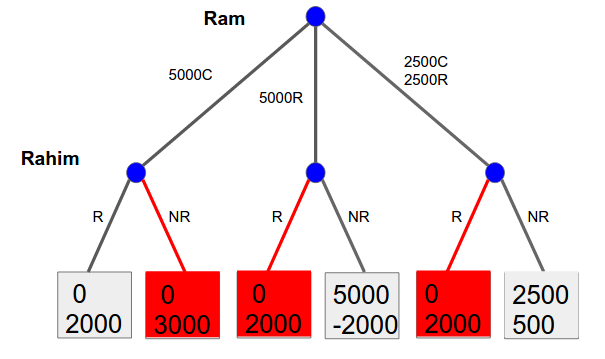
\includegraphics[width=1\columnwidth]{1_gt2.png}
\caption{Backward Induction: Rahim}
\label{1_gt2}


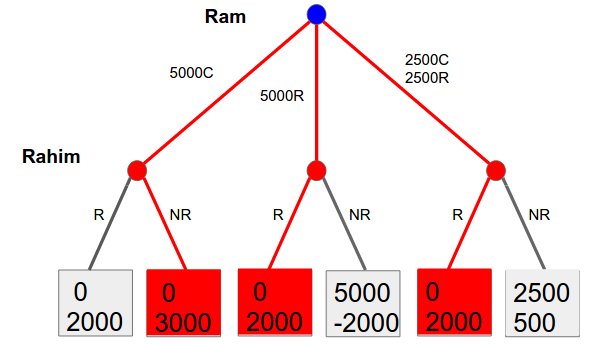
\includegraphics[width=1\columnwidth]{1_gt3.png}
\caption{Backward Induction: Ram}
\label{1_gt3}
\end{multicols}
\end{figure}

\section{Watergate scandal}
\textbf{(a)} \\
If the decision is \emph{6-2}, then it is better for the president to defy rather than comply, arguing that the split decision can not bind him. But, in this case the Court would not have enough evidence to prosecute him, hence they are worse off. If the decision is \emph{8-0}, then the president has to comply because if he defies, then it would probably lead to his impeachment. Thus, the payoff for comply is better than defy. Also, if he complies, then the Court would have enough evidence to prosecute, thus their payoff is better in this case.\\
\textbf{(b)}
\begin{figure}[h!]
\centering
\begin{multicols}{3}
\label{2_gt1}
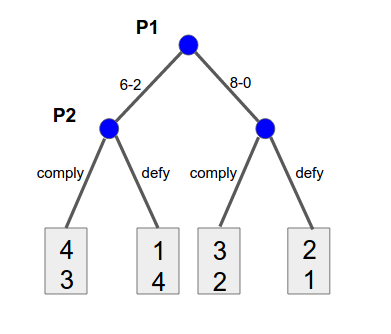
\includegraphics[width=1\columnwidth]{2_gt1.png}
\caption{Game Tree}


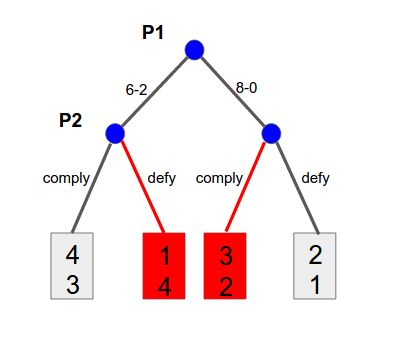
\includegraphics[width=1\columnwidth]{2_gt2.png}
\caption{Backward Induction: Player 2}
\label{2_gt2}


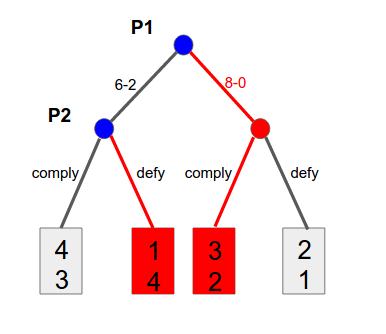
\includegraphics[width=1\columnwidth]{2_gt3.png}
\caption{Backward Induction: Player 1}
\label{2_gt3}
\end{multicols}
\end{figure}

By Backward Induction, \emph{Player 2 argues} that if the decision is \emph{6-2}, then it is better to \emph{defy}, since $4$ is better than $3$. If the decision, is \emph{8-0}, then it is better to \emph{comply}, since $2$ is better than $1$. This is illustrated in Figure \ref{2_gt2}. Now, \emph{Player 1 argues} that if the decision is \emph{6-2}, then Player 2 will \emph{defy} and the payoff is $1$. But, if the decision is \emph{8-0}, then Player 2 will comply and the payoff is $3$. Therefore, \emph{8-0} is better(Figure \ref{2_gt3}). \\ \\
Thus, the predicted outcome is \emph{\{ 8-0, comply \}}. \\ \\
\textbf{(c)} \\
Nixon could have a better outcome if he had successfully influenced the 2 judges to give the decision in his favour and then defy the judgement, arguing that a split decision can not bind the President. His payoff would then be 4 instead of 2.\\ \\
\textbf{(d)} \\
The Supreme Court gave an \emph{8-0} decision and the President had to comply and hand-over the tapes(he also resigned after 16 days).
\section{Campus Shops}
\textbf{(a)} Let the price chosen by $S1$ be $p_1$, then if $S2$ choses $p_2$, the revenue generated by $S1$ and $S2$ is: 
$$\pi_{1} = p_1 \times (10-2p_1-p_2)$$
$$\pi_{2} = p_2 \times (10-p_1-2p_2)$$
Now, given $p_1$, $S2$ will choose $p_2$ such that $\pi_2$ is maximum, or:
$$\frac{\partial \pi_2}{\partial p_2}= 0$$
$$ 10 - p_1 -4p_2  = 0$$
$$p_2 = \frac{10-p_1}{4}$$
Now, since $S1$ knows the above strategy of $S2$, it will choose $p_1$, such that $\pi_1$ is maximum, given the above value of $p_2$:
$$\frac{\partial \pi_1}{\partial p_1}= 0$$
$$\frac{\partial}{\partial p_1}\Big(10p_1 - 2p_1^2 -p_1(\frac{10-p_1}{4})\Big)= 0$$
$$10 - 4p_1 - 10/4 + p_1/2 = 0$$
$$p_1 = 15/7 \sim 2.14$$
Therefore $p_2 = 55/28 \sim 1.96$. Thus, revenues are $\pi_1 = 8.03$ and $\pi_2 = 7.72$ 
\newpage
\textbf{(b)} \\ \\
From the scenario of S1, if S1 chooses $p_1 < 0$, then $\pi_1= p_1a_1 < 0$. Thus, S1 always chooses $p_1 > 0 $. \\
Now, if $p_1>5$, then since $p_2 > 0$(S2 always reasons similarly), $a_1 = 0$. Then, $\pi_1=0$. \\
Therefore, S1 always chooses $0 \leq p_1 \leq 5$. \\
Since S2 reasons similarly, $0 \leq p_2 \leq 5$. \\ \\
\textbf{(c)} \\ \\
Since $\pi_1 = a_1p_1$, therefore \\
$$\pi_1 = 10p_1 - 2p_1^2 - p_2p_1 \times \mathds{1}[2p_1+p_2<10]$$
Similarly,
$$\pi_2 = 10p_2 - 2p_2^2 - p_2p_1 \times \mathds{1}[2p_2+p_1<10]$$
where $\mathds{1}[f]$ returns 1 if \emph{f} is true, otherwise 0. \\
\textbf{(d)} \\ 
\begin{figure}[h!]
\begin{center}
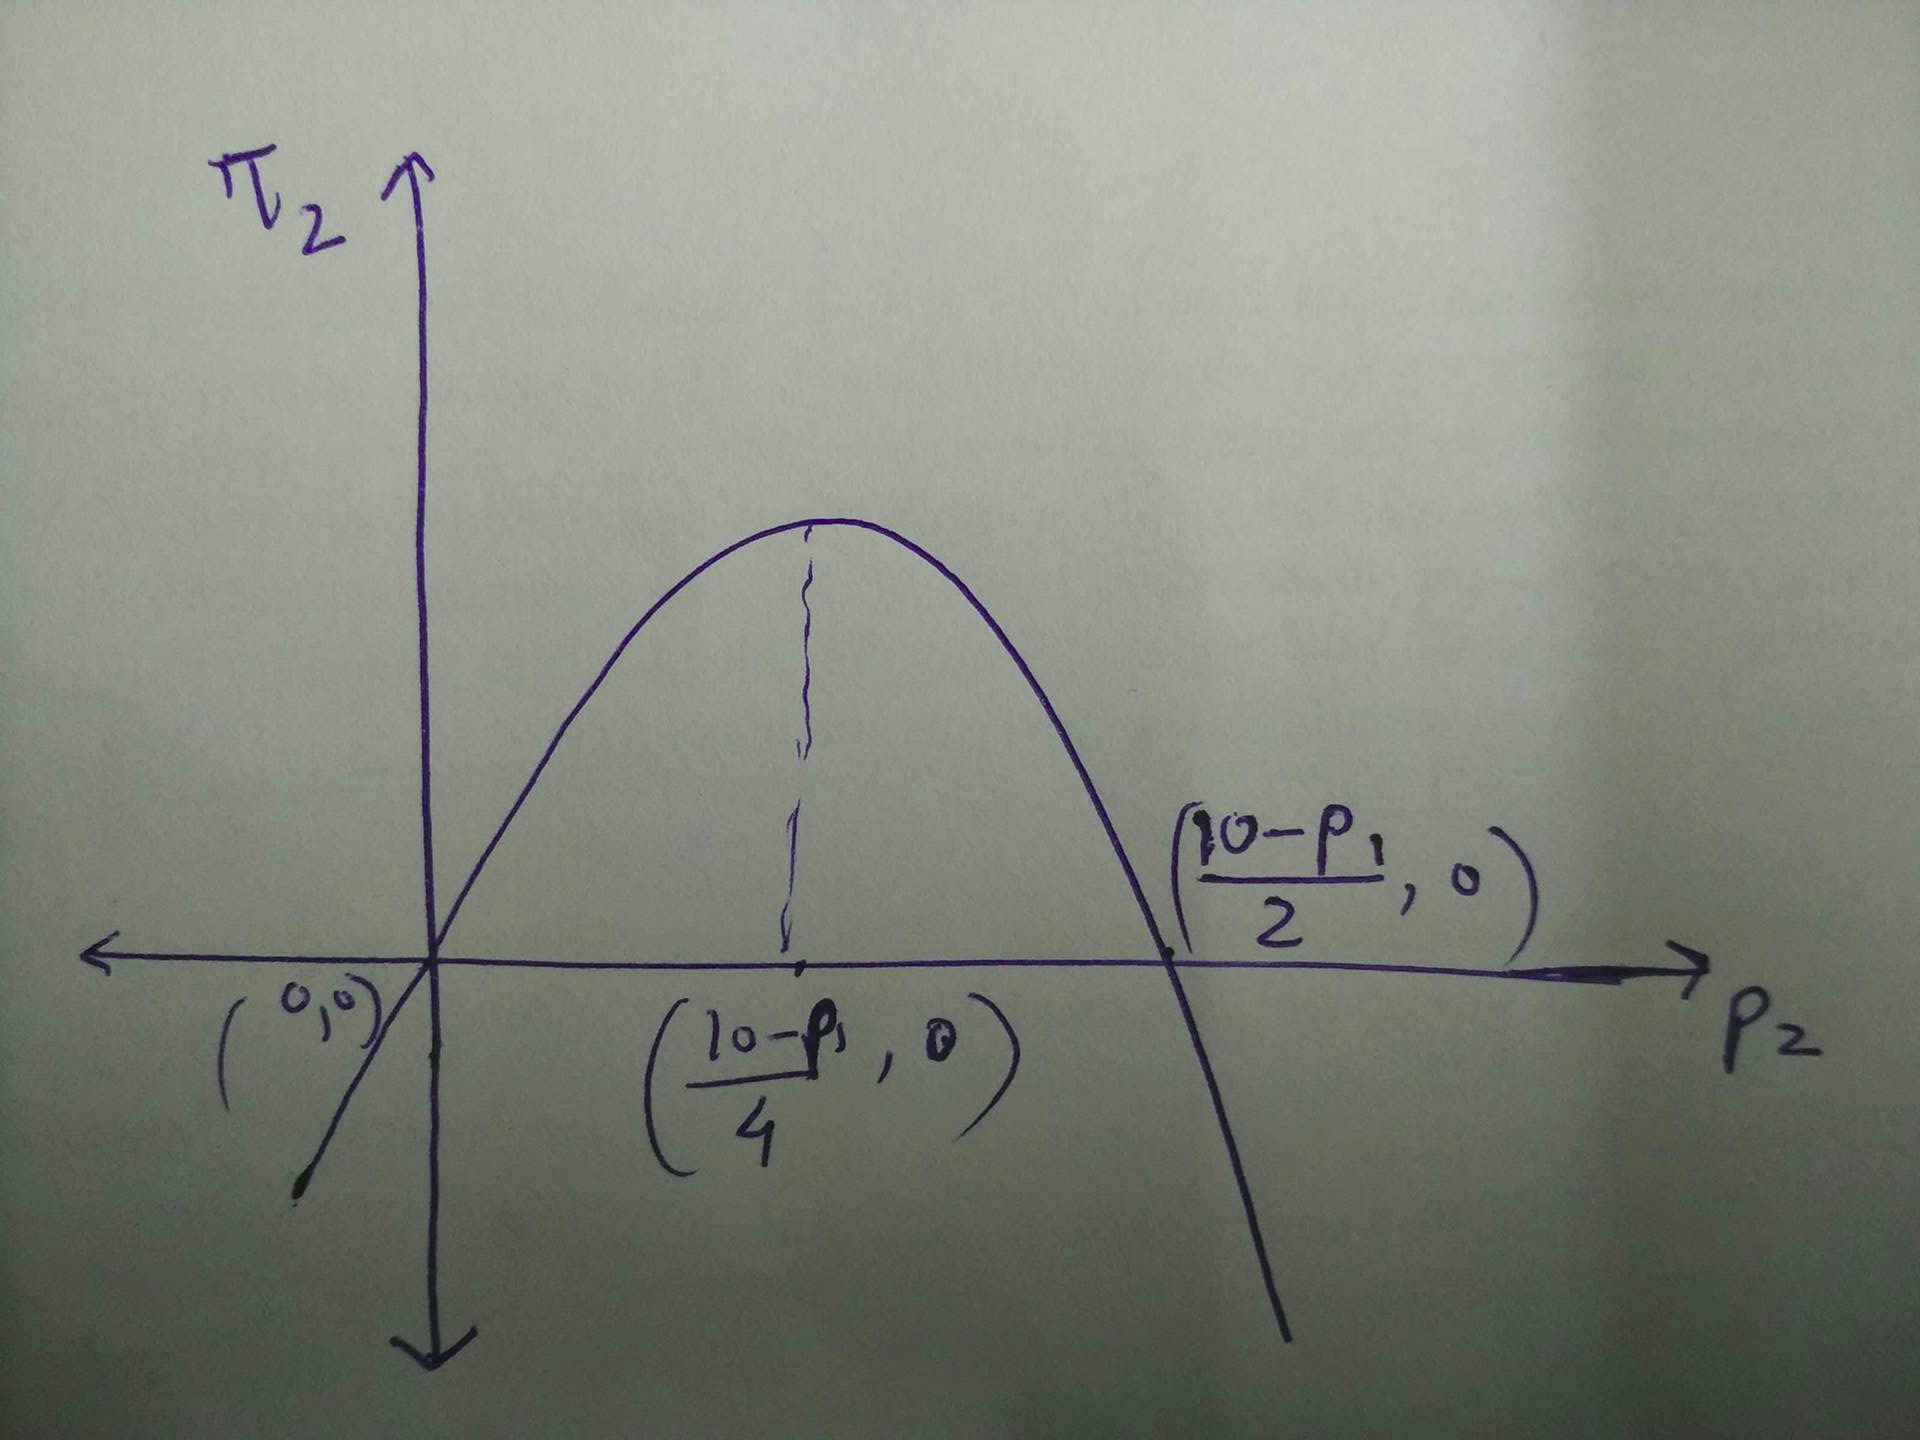
\includegraphics[scale=0.1]{quad1.png}
\label{qu}
\caption{$\pi_2(p_1,p_2)$}
\end{center}
\end{figure}
Consider the following graph(Figure 7), where $y = \pi_2(p_1,p_2)$ 
$$\pi_2 = 10p_2 - 2p_2^2 - p_2p_1$$
\textbf{(e)} \\
Best Response Function $f(p_1)$ is given by :
$$\frac{\partial \pi_2}{\partial p_2}= 0$$
$$p_2 = \frac{10-p_1}{4}$$
\textbf{(f)} \\
Consider the graph (Figure 8), 
$$\pi_1(p_1, f(p_1)) = \frac{-7p_1^2+30p_1}{4}$$
\begin{figure}[h!]
\begin{center}
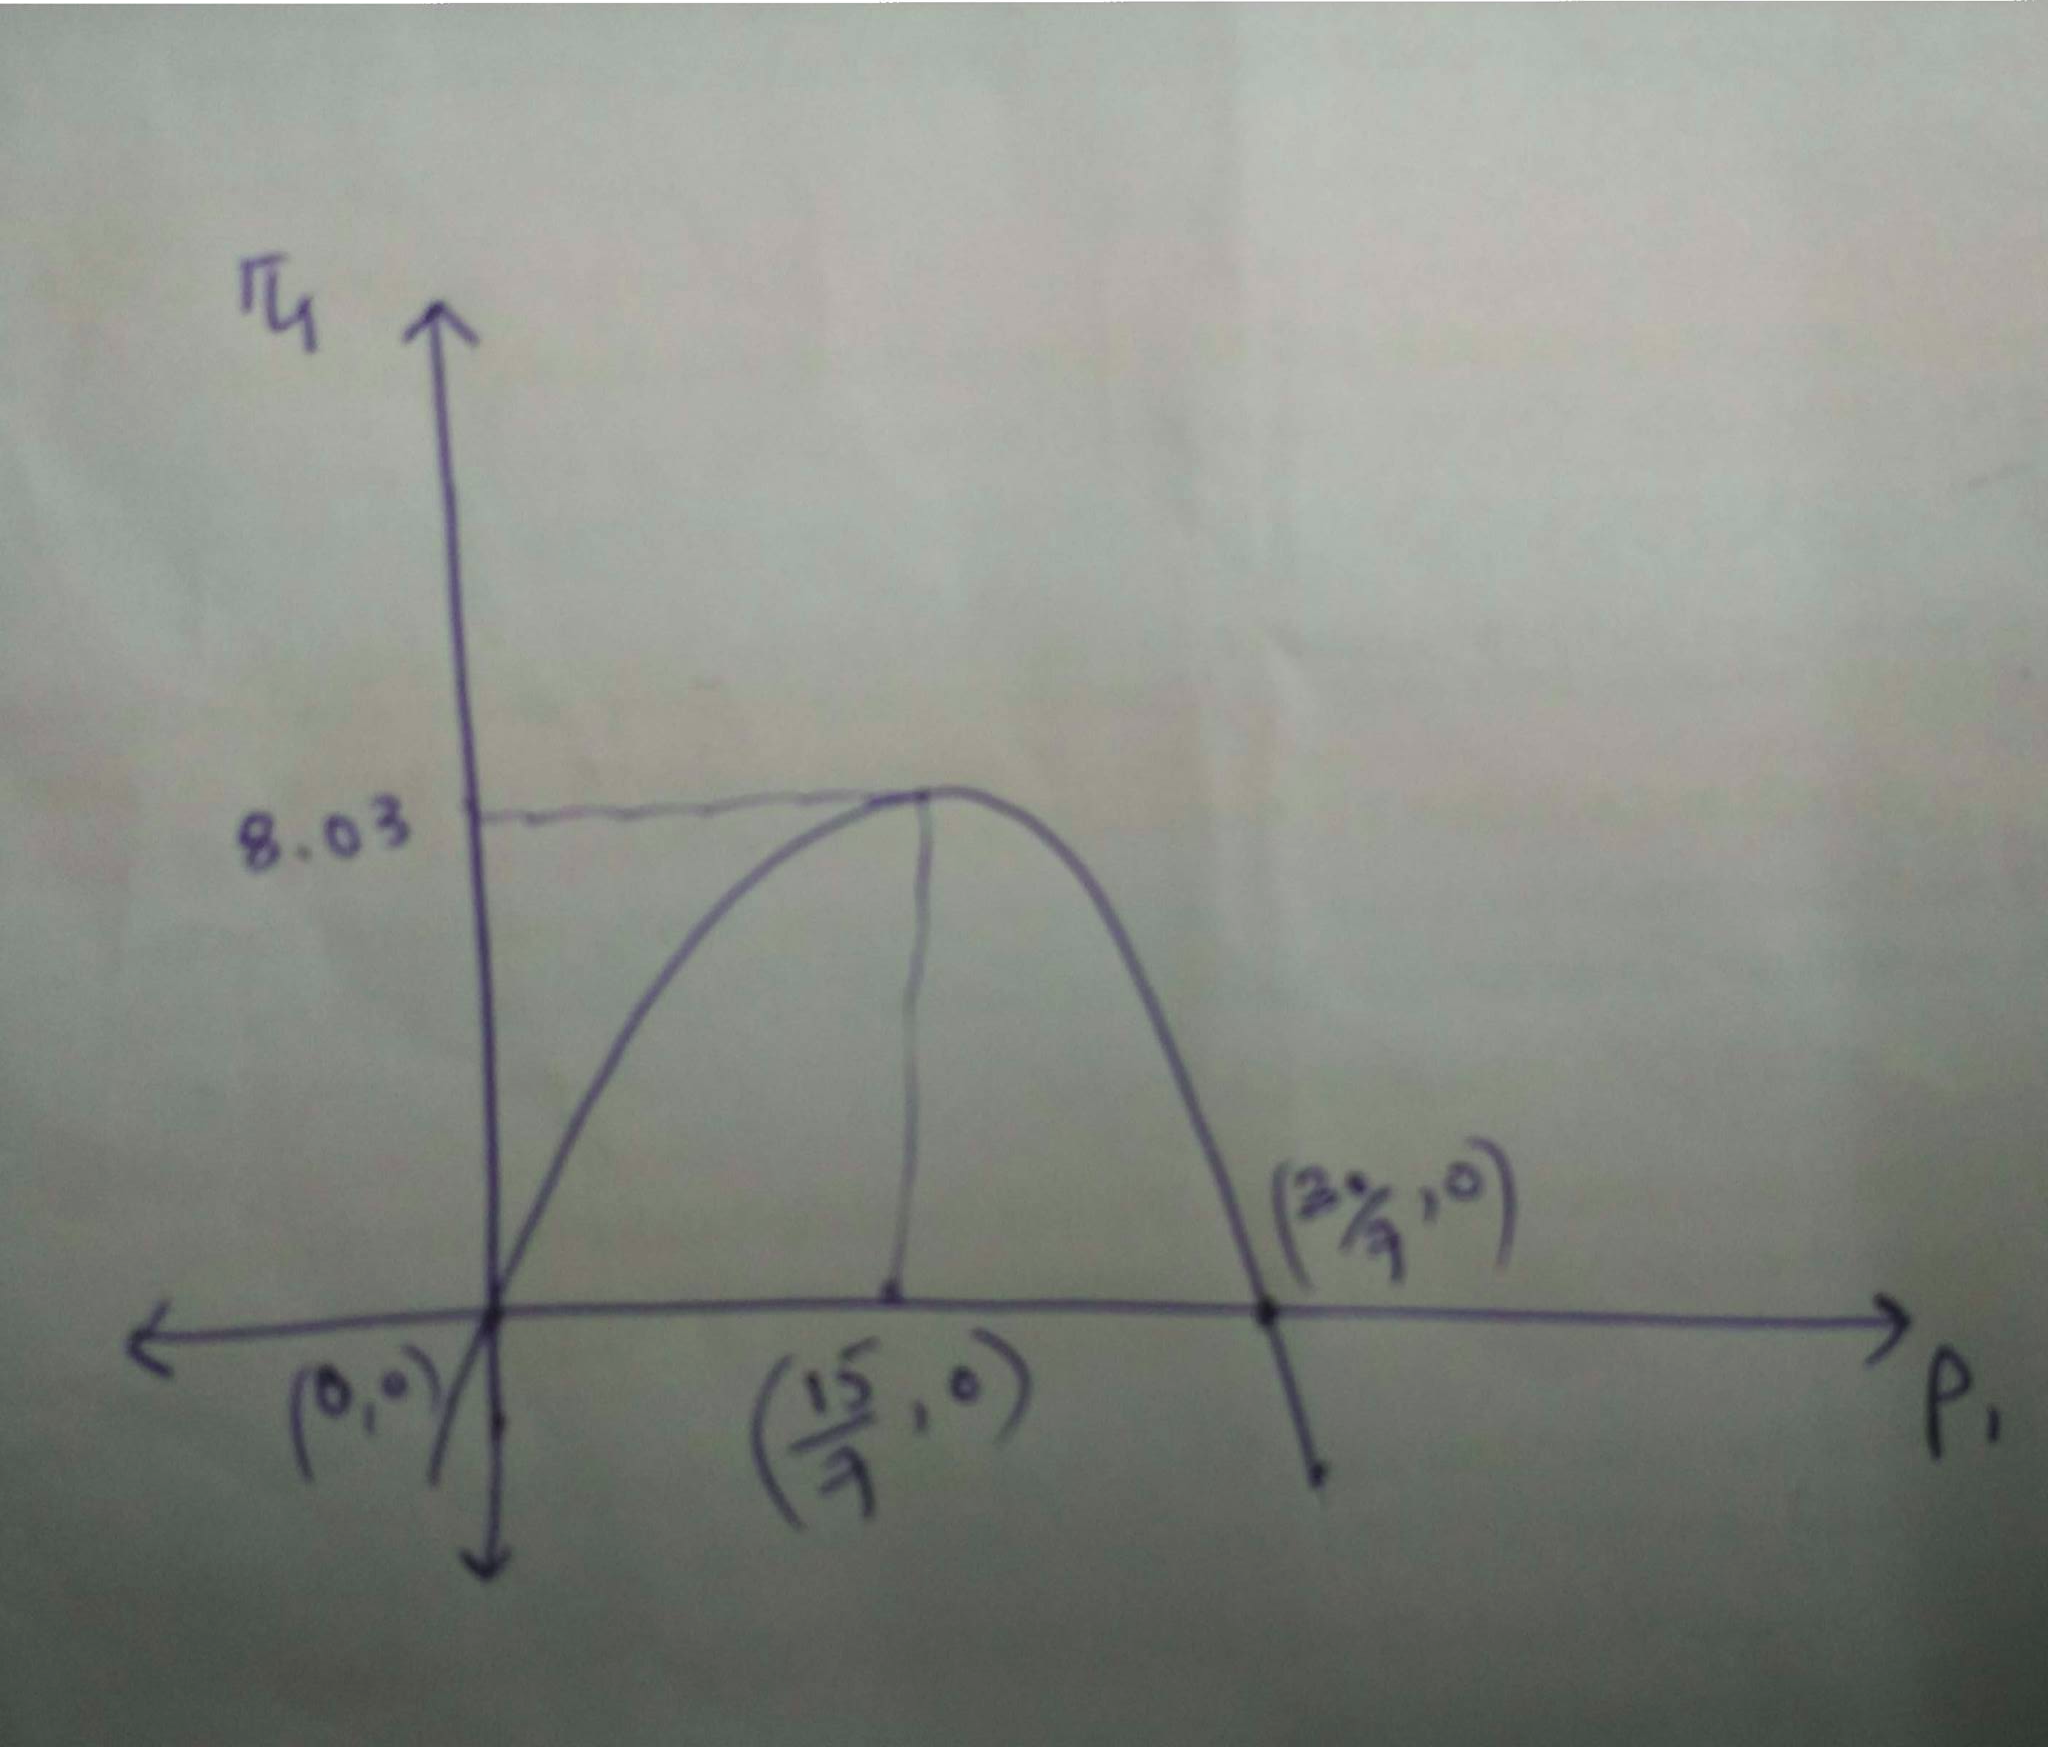
\includegraphics[scale=0.1]{quad2.png}
\label{qu2}
\caption{$\pi_1(p_1, f(p_1))$}
\end{center}
\end{figure}
This is maximum at $p_1$, such that:
$$\frac{\partial \pi_1}{\partial p_1}= 0$$
$$p_1 = \frac{15}{7}$$
\section{Tax Rate}
Suppose the government(Player 1) announces a tax rate $r$, and the citizens(Player 2) put effort $e$, then the respective payoff are:
$$ \pi_1 = r \times (4e - 4re - e^2)$$
$$ \pi_2 = (1-r) \times (4e - 4re - e^2)$$
Given $r$, citizens would put effort $e$, such that their payoff($\pi_2$) is maximum:
$$\frac{\partial \pi_2}{\partial e}= 0$$
$$ 4(1-r)- 4r(1-r) - 2(1-r)e = 0$$
$$e = 2(1- r), r \neq 1$$
Since the government would know the above strategy of the citizens, it would choose r such that their payoff ($\pi_1$) is maximum, given the above the value of e:
$$\frac{\partial \pi_1}{\partial r}= 0$$
$$\frac{\partial}{\partial r}\Big(r \times (8(1-r) - 8r(1-r) - 4(1-r)^2)\Big)= 0,r \neq 1$$
$$\frac{\partial}{\partial r}\Big(4r - 8r^2+4r^3\Big)= 0,r \neq 1$$
$$1 - 4r + 3r^2 = 0,r \neq 1$$
$$r = 1/3$$
Thus, the government would choose $r=1/3$ to maxmize it's payoff.
\section{Wireless Spectrum Block}
\textbf{(a)} \\
Payoff function for player \emph{i} is:
$$ \pi_i = (v_i-h_i) \times \mathds{1}[b_i>h_i] $$
where $\mathds{1}[f]$ returns 1 if \emph{f} is true, otherwise 0. Clearly, this is positive for only the player with the highest bid and 0 for the rest of the players. Thus, the n-tuple(for n players) for the payoff  function is as follows:
$$\pi(b_1,...,b_n) = \{(v_1-h_1) \times \mathds{1}[b_1>h_1], ... ,(v_n-h_n) \times \mathds{1}[b_n>h_n]\}$$
Clearly, $\pi(b_1,...,b_n)$ is a 1-hot vector.\\ \\
\textbf{(b)} \\
Consider the scenario from the persective of the $i^{th}$ player. There are three cases for player i's bid($b_i$): \\ \\
\emph{Case 1:} $b_i < v_i$, In this case, player i will look to submit a bid such that $b_i > h_i$. But, this is not possible as there can always be $h_i$, such that $ b_i < h_i < v_i$. \\ \\
\emph{Case 2:} $b_i > v_i$, Here, there can be three subcases: \\
\emph{Subcase 1:} $h_i > b_i$, player i does not win in this case and $\pi_i = 0$. So, $b_i$ does not matter.\\
\emph{Subcase 2:} $h_i < v_i$, player i wins and $\pi_i = v_i-h_i$. So, So, $b_i$ does not matter.\\
\emph{Subcase 3:} $v_i < h_i < b_i$, player i wins but $\pi_i = v_i-h_i < 0$. He/She could have been better off had he/she lost, because then $\pi_i = 0$, which is better than negative. \\ \\
So, by the above analysis, we conclude that player i is worse off for both the cases, when $b_i< v_i$ and $b_i > v_i$. Thus, the best response choice for player i is $b_i = v_i$.

\section{Demonetised Note Auction}
\textbf{(a)} \\
Payoff Function is given by:
$$\pi_i(b_i,h_i) = (v_i-b_i) \times \mathds{1}[b_i > h_i]$$
where $\mathds{1}[f]$ returns 1 if \emph{f} is true, otherwise 0. The above simply says, that if player i's bid, $b_i$, is higher than the bid $h_i$, then the payoff is ($v_i-b_i$), otherwise 0.\\ \\
\textbf{(b)} \\
\emph{Case 1} $b_i< (v_i-1)$ \\
In this case there can always be $h_i$, such that $h_i=(v_i-1)$. Then the player i will lose the auction and $\pi_i = 0$. \\ \\
\emph{Case 2} $b_i > v_i$ \\
In this case, even if player i wins election, then payoff $\pi_i = v_i - b_i < 0$, which is worse than losing the election. \\ \\
Thus, by analysing the above two cases, we can say that $v_i,(v_i-1) \succeq b_i$. \\ \\
\textbf{(c)} \\
Since there can be no $h_i$, such that $(v_i-1)< h_i < v_i$. So, the result of the auction is going to be same for both the cases with respect to player i. But, payoff for strategy $v_i$, $\pi_i = 0$ and for strategy $v_i-1$. $\pi_i = 1$, which is better than the former. \\ \\
Therefore, $(v_i-1) \succeq v_i$.
\end{document}


